\chapter{Materiais e Métodos}
\label{cap:03}

Para a prototipagem do traçador I-V houve a necessidade de se seguir as seguintes etapas:
\begin{itemize}
	\item Integração entre os componentes do protótipo sendo eles:
	\begin{itemize} 
		\item Arduino;
		\item Carga eletrônica;
		\item Painel solar;
		\item Sensor ADS1115;
		\item Cartão SD.
	\end{itemize}
	\item Teste de precisão na coleta de dados;
	\item Padronização e fixação do ambiente de testes;
	\item Teste do protótipo;
	\item Armazenamento da amostragem coletada;
	\item Análise e tratamento da amostra;
	\item Verificação e resolução de erros e/ou problemas.

\end{itemize}

\subsection{Arduino}
A plataforma Arduino foi utilizada de maneira centralizar o controle de todos os periféricos necessários para a prototipagem. Foi utilizado as saídas PWM, Barramento I2C e SPI.

IMAGEM que será adicionada
%Imagem ARduino+I2C+SPI

\subsection{I2C e SPI}
As comunicações I2C e SPI permitiram o uso de ferramentas não disponíveis no hardware original do Arduino, como a utilização de um ADC de 16bits ou do cartão SD para armazenamento dos dados.

Imagem SDCARDMOD

\subsection{Carga Eletronica}
A carga eletrônica permitiu a variação dos valores de corrente e tensão do painel, fator indispensável para a ação do traçador.

Imagem Carga eletrônica

\subsection{Circuito Completo}

Se observa na figura~\ref{fig:Circuito} como se assemelha o circuito eletrônico completo do traçador de curvas I-V.


\FloatBarrier
\begin{figure}[!htbp]
	\centering
	%scale redimensiona a figura.
	%1.5 = 150% do tamanho original
	%1 = 100% do tamanho original
	%0.20 = 20% do tamanho original
	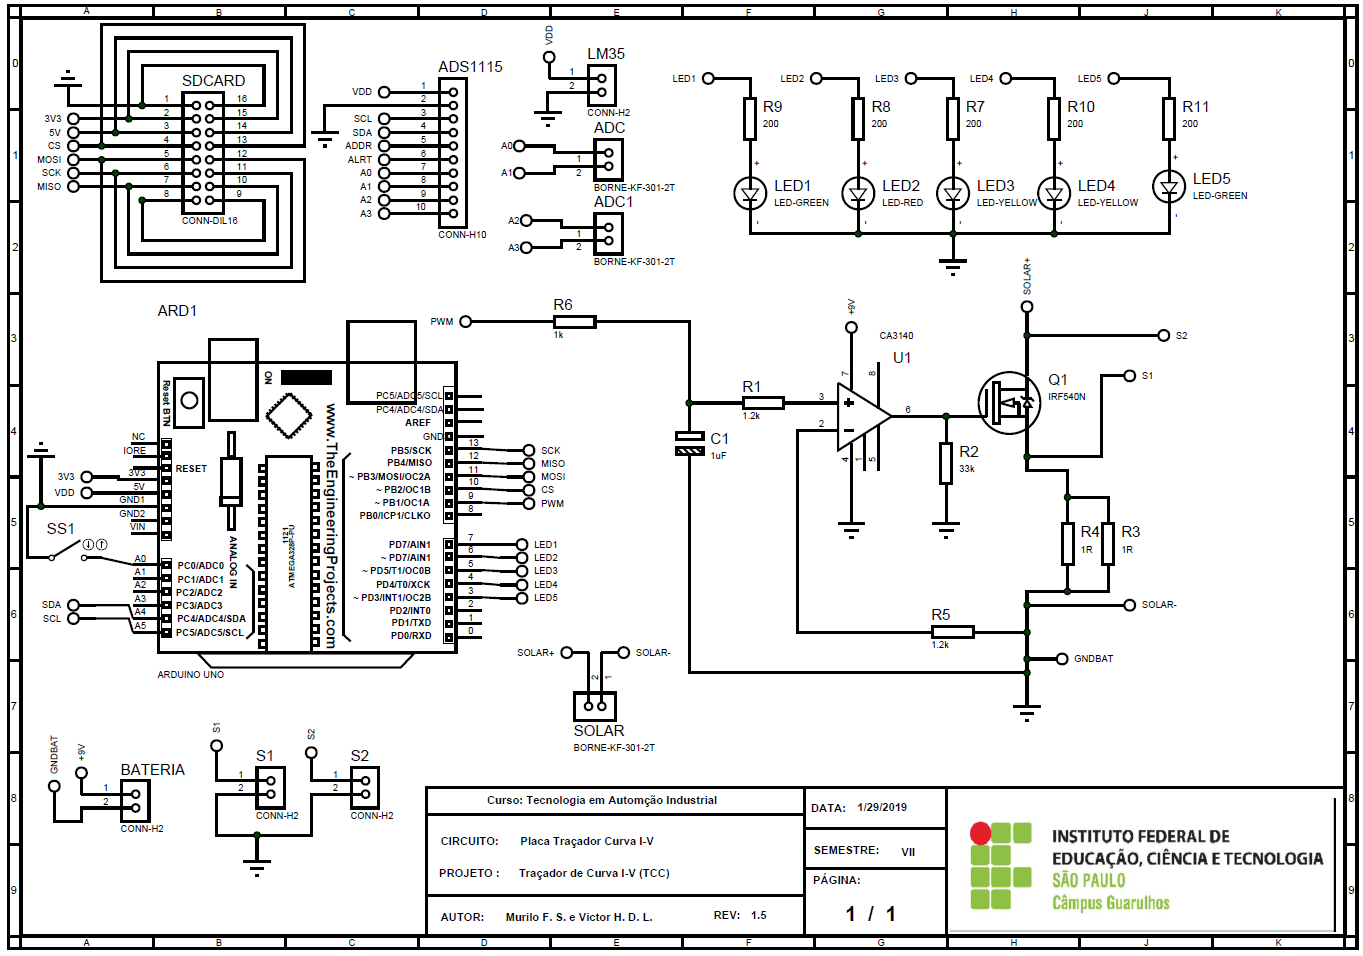
\includegraphics[scale=0.3]{imagens/CircuitoCompleto.png}
	\caption{Circuito eletrônico completo. Fonte: Elaborado pelo Autor. 	}
	\label{fig:Circuito}
\end{figure}
\FloatBarrier

O circuito pode ser separado em diversas partes que serão separadas em:
\begin{enumerate}
	\item Conexões com o Arduino;
	\item Conexões Módulos;
	\item Carga Eletrônica;
	\item LEDs para sinalização.
\end{enumerate}

	
\subsubsection{Conexões com o Arduino}

A primeira parte do circuito,  figura~\ref{fig:CircuitoArduino}, as entradas e saídas disposta pelo Arduino e utilizadas para os acionamentos e sensoriamentos.

\begin{figure}[!htbp]
	\centering
	%scale redimensiona a figura.
	%1.5 = 150% do tamanho original
	%1 = 100% do tamanho original
	%0.20 = 20% do tamanho original
	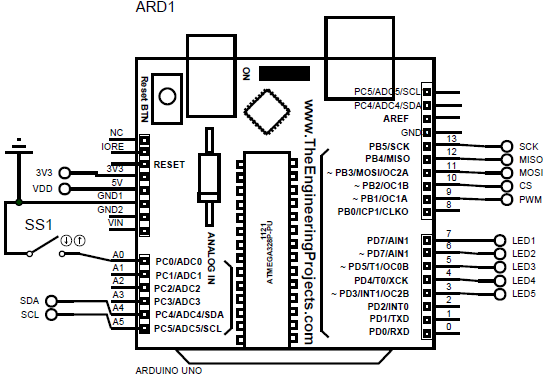
\includegraphics[scale=1.0]{imagens/CircuitoArduino.png}
	\caption{Circuito eletrônico, foco no componentes mais próximos ao Arduino. Fonte: Elaborado pelo Autor. 	}
	\label{fig:CircuitoArduino}
\end{figure}
\FloatBarrier

Na figura~\ref{fig:CircuitoArduino} se observa as conexões de alimentação dos módulos, os pinos das conexões de diferentes redes, sendo elas I2C e SPI. Há também os pinos conectados aos LEDs e ao botão que inicia o processo.

\subsubsection{Conexões Módulos}

A segunda parte do circuito,  figura~\ref{fig:CircuitoMod}, desrespeito aos conectores que serão utilizados para os módulos auxiliares para o processo da carga eletrônica.

\begin{figure}[!htbp]
	\centering
	%scale redimensiona a figura.
	%1.5 = 150% do tamanho original
	%1 = 100% do tamanho original
	%0.20 = 20% do tamanho original
	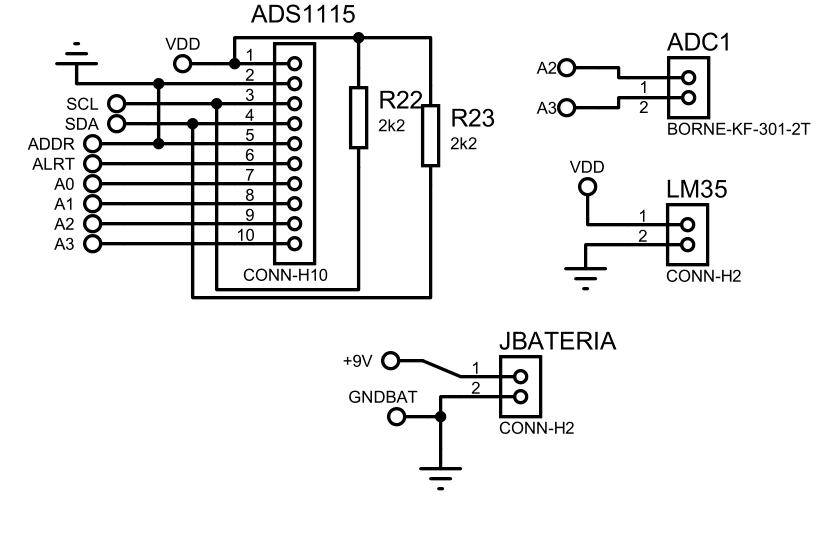
\includegraphics[scale=0.7]{imagens/CircuitoMod.png}
	\caption{Circuito eletrônico, foco nas conexões com o módulo. Fonte: Elaborado pelo Autor. 	}
	\label{fig:CircuitoMod}
\end{figure}
\FloatBarrier

Na figura~\ref{fig:CircuitoMod} se observa as conexões para os módulos, Cartão SD e ADS1115, além de conexões auxiliares para a o LM35, sensor de temperatura e para os sinais de entrada do módulo ADS1115.

\subsubsection{Carga Eletrônica}

A terceira parte do circuito,  figura~\ref{fig:CircuitoElet}, a carga eletrônica, principal circuito para o funcionamento do protótipo.

\begin{figure}[!htbp]
	\centering
	%scale redimensiona a figura.
	%1.5 = 150% do tamanho original
	%1 = 100% do tamanho original
	%0.20 = 20% do tamanho original
	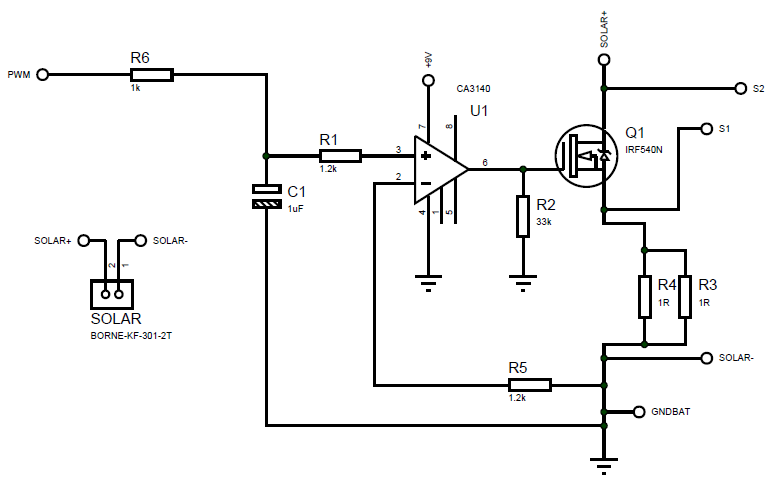
\includegraphics[scale=0.7]{imagens/CircuitoElet.png}
	\caption{Circuito eletrônico, foco na carga eletrônica. Fonte: Elaborado pelo Autor. 	}
	\label{fig:CircuitoElet}
\end{figure}
\FloatBarrier

Na figura~\ref{fig:CircuitoElet} se observa os componentes para o uso da carga eletrônica. Há também a presença dos conectores para os cabos provenientes do painel solar.

\subsubsection{Conjunto de LEDs}

A parte final do circuito,  figura~\ref{fig:CircuitoLED}, o conjunto de LEDs, \textit{Light-Emitting Diode}, Diodo Emissor de Luz, o qual tem como principal função garantir uma interface visual para o usuário, permitindo assim se encontrar durante o processo e erros ocorridos.

\begin{figure}[!htbp]
	\centering
	%scale redimensiona a figura.
	%1.5 = 150% do tamanho original
	%1 = 100% do tamanho original
	%0.20 = 20% do tamanho original
	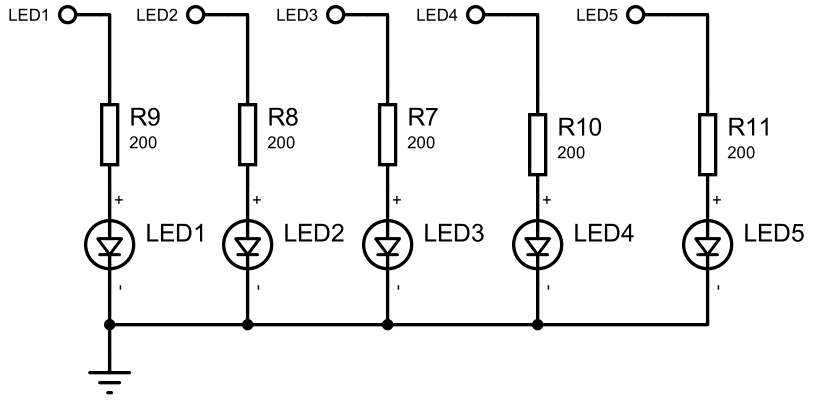
\includegraphics[scale=1.0]{imagens/CircuitoLED.png}
	\caption{Circuito eletrônico, foco no conjunto de LEDs. Fonte: Elaborado pelo Autor. 	}
	\label{fig:CircuitoLED}
\end{figure}
\FloatBarrier

Na figura~\ref{fig:CircuitoLED} se observa os cinco LEDs utilizados para o informativo ao usuário.

\subsection{Métodos}
\subsubsection{Controle de Variáveis}
Durante os experimentos foram necessários atestar alguns aspectos, garantindo maior estabilidade no processo de aquisição de dados:
\begin{itemize}
\item Irradiância solar fixa;
\item Uso de sensores precisos.
\end{itemize}

Para garantir maior veracidade e precisão na coleta de dados, foi realizado um teste com 30 diferentes valores a serem coletados pelo sensor utilizando ADS1115 e um multímetro de alta precisão. Ao se comparar os dados do multímetro e do ADS1115, nota-se os valores correspondentes do sensor em relação ao multímetro, como pode ser observado na figura~\ref{fig:Precisao}.

\FloatBarrier
\begin{figure}[!htbp]
	\centering
	%scale redimensiona a figura.
	%1.5 = 150% do tamanho original
	%1 = 100% do tamanho original
	%0.20 = 20% do tamanho original
	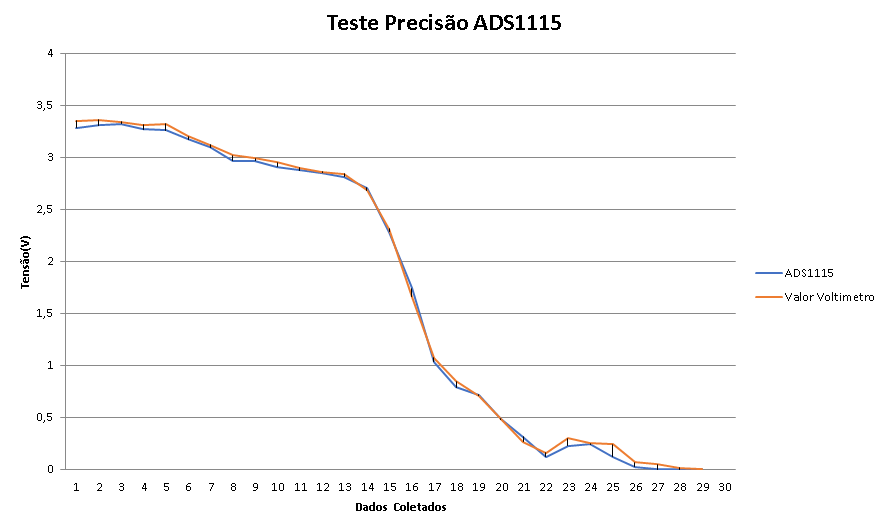
\includegraphics[scale=1.0]{imagens/Precisao}
	\caption{30 diferentes valores de tensão e comparação entre o sensor e um multímetro comercial. Fonte: Elaborado pelo Autor. 	}
	\label{fig:Precisao}
\end{figure}
\FloatBarrier

Considerando o clima e tempo instável oscilando entre dias chuvosos, nublados e alguns ensolarados, houve a necessidade de uma maneira de viabilizar os testes ainda que houvesse clima desfavorável. O engenho que permitiu tal feito foi o uso de uma lâmpada halogênea, que teve como papel gerar e simular a mesma irradiância que seria gerada pelo Sol em um dia sem nuvens.  

Imagem Da Lampada
...

\subsubsection{Comportamento do Protótipo}

De maneira a tornar o uso do traçador mais acessível e funcional, foram instalados LEDs que apresentam em qual parte do processo de aquisição de dados o traçador se encontra, e um LED para sinalização de erros durante a aquisição de dados, sendo suas cores:

\begin{itemize}
	\item Amarelo;
	\item Branco;
	\item Verde 1;
	\item Verde 2;
	\item Vermelho.
\end{itemize}

Foram utilizadas diferentes combinações de LEDs para sinalizar as diferentes etapas, assim como  reproduzido na tabela~\ref{tab:LEDS}.

\FloatBarrier
\begin{table}[!htbp]
	\centering
	\caption{Combinação dos LEDs de sinalização}
	\begin{tabular}{ c | c }
		\hline
		\textbf{Combinações de Cores} & \textbf{Função}                                   \\ \hline
		Vermelho                      & Erro durante a coleta                             \\ \hline
		Amarelo,Verde1                & Aguardando habilitação pelo usuário para a coleta \\ \hline
		Verde2                        & Coleta de dados habilitada                        \\ \hline
		Branco                        & Coletando de dados                                \\ \hline
		Branco,Verde1,Vermelho        & Finalização da coleta                             \\ \hline
	\end{tabular}
	\\ \vspace{0.2cm}
	\textbf{Fonte:} Elaborada pelo autor
	\label{tab:LEDS}
\end{table}
\FloatBarrier

Ao se utilizar da interface através dos LEDs foi possível tornar a coleta de dados mais dinâmica, de maneira a facilitar o uso do usuário e a verificação das etapas e o possível aparecimento de erros.

Tendo a interface pronta, e o circuito montado pronto para os testes, houve então a primeira verificação. Os primeiros experimentos foram feitos utilizando uma \textbf{Resistência \textit{Shunt}}(RS) de aproximadamente 3 Ohms, o que causou uma grande deformação na curva proveniente dos valores coletados.

Após novos testes com diferentes resistências, foi  possível chegar ao resultado mais próximo do esperado ao se utilizar dois resistores de 1 Ohm em paralelo. Houve também a necessidade de alterar alguns pontos da programação tendo a finalidade de se obter mais pontos e garantir uma melhor resolução da curva.



